\begin{figure}
    \centering
    \setlength{\tabcolsep}{1pt}
    {\small
    \begin{tabular}{cccccc}
        \raisebox{28pt}{\rotatebox[origin=t]{90}{Input}}& 
        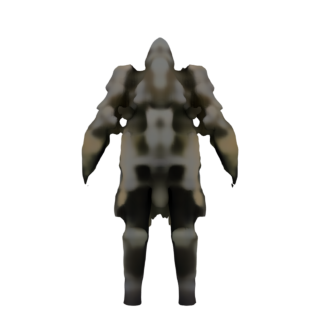
\includegraphics[width=0.32\linewidth]{images/ablation_plot/shap_e/mv_0_image_tile_1.png} &
        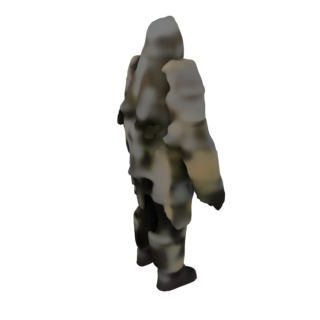
\includegraphics[width=0.32\linewidth]{images/ablation_plot/shap_e/mv_0_image_tile_2.png} &
        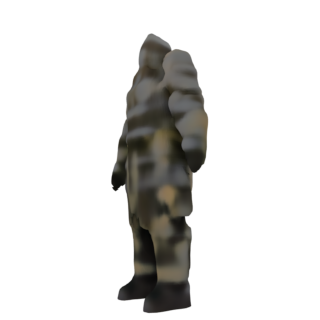
\includegraphics[width=0.32\linewidth]{images/ablation_plot/shap_e/mv_0_image_tile_5.png} \\
        %
        \raisebox{28pt}{\rotatebox[origin=t]{90}{w/o text prompt}} & 
        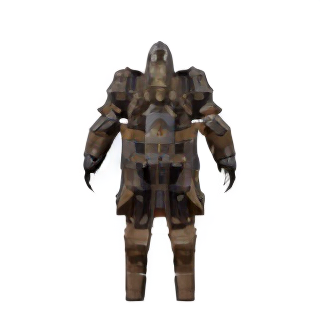
\includegraphics[width=0.32\linewidth]{images/ablation_plot/no_prompt/no_prompt_tile_1.png} &
        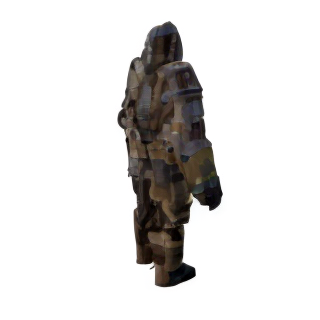
\includegraphics[width=0.32\linewidth]{images/ablation_plot/no_prompt/no_prompt_tile_2.png} &
        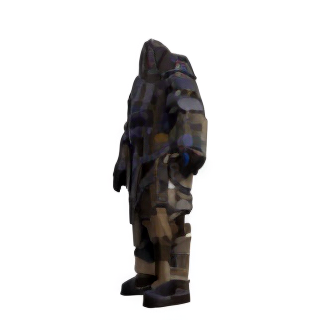
\includegraphics[width=0.32\linewidth]{images/ablation_plot/no_prompt/no_prompt_tile_5.png} \\
        %
        \raisebox{28pt}{\rotatebox[origin=t]{90}{w/o diverse lighting}} &
        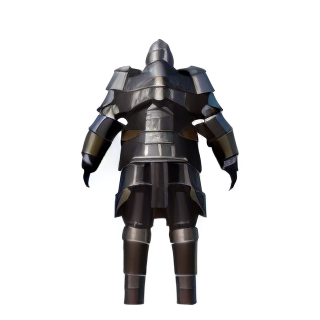
\includegraphics[width=0.32\linewidth]{images/ablation_plot/single_hdr/single_source_tile_1.png} &
        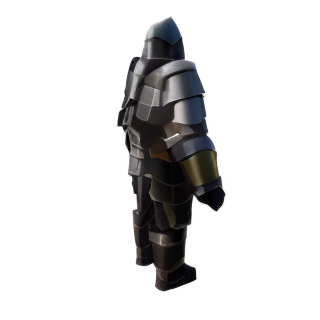
\includegraphics[width=0.32\linewidth]{images/ablation_plot/single_hdr/single_source_tile_2.png} &
        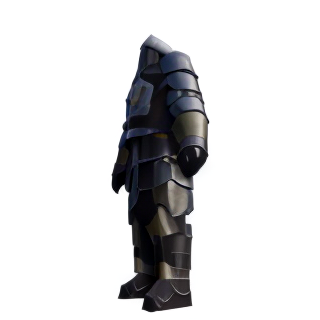
\includegraphics[width=0.32\linewidth]{images/ablation_plot/single_hdr/single_source_tile_5.png} \\
        %
        \raisebox{28pt}{\rotatebox[origin=t]{90}{Full Model}} &
        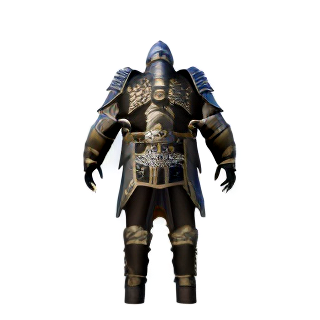
\includegraphics[width=0.32\linewidth]{images/ablation_plot/full/full_tile_1.png} &
        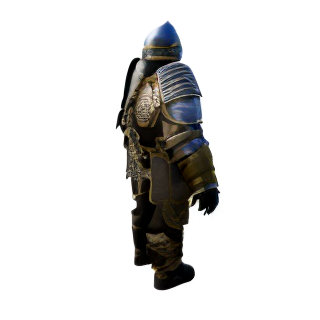
\includegraphics[width=0.32\linewidth]{images/ablation_plot/full/full_tile_2.png} &
        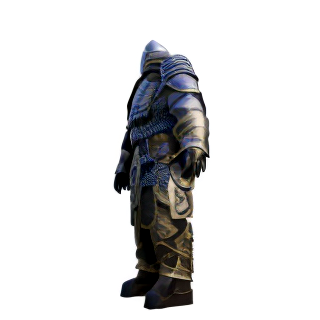
\includegraphics[width=0.32\linewidth]{images/ablation_plot/full/full_tile_5.png} \\
        %
        & \multicolumn{3}{c}{``A knight in full plate armor''}
        %
    \end{tabular}
    }
    \caption{Qualitative ablation study of our method for generating “A knight in full plate armor,” demonstrating the impact of different model components. The top row shows the coarse input shape generated without refinement. Subsequent rows show the effects of removing specific components: omitting the text prompt leads to reduced texture detail, while excluding diverse lighting results in a flatter appearance with less realistic shading. The full model (bottom row) achieves the most refined and detailed result, preserving intricate armor details and realistic lighting across multiple views, highlighting the importance of each component in producing high-quality outputs.}
    \label{fig:ablation}
\end{figure}